
% ----------------------------------------------------------------------
%  Set the document class
% ----------------------------------------------------------------------
\documentclass[11pt,a4paper,twoside]{article}

% ----------------------------------------------------------------------
% Define external packages, language, margins, fonts and new commands
% ----------------------------------------------------------------------
%\input{preamble} 
\usepackage[utf8]{inputenc}   % <<<<< Linux
\usepackage[english]{babel} % <<<<< English
\usepackage{notoccite}
\usepackage[skip=0.5\baselineskip]{caption}
\hyphenation{GTKWave}
\usepackage{listings}
\usepackage[all]{nowidow}

%blind text
\usepackage{lipsum}

\usepackage{graphicx}
\graphicspath{ {./} {../../figlib/} }
\def\FontLn{% 16 pt normal
  \usefont{T1}{phv}{m}{n}\fontsize{16pt}{16pt}\selectfont}
\def\FontLb{% 16 pt bold
  \usefont{T1}{phv}{b}{n}\fontsize{16pt}{16pt}\selectfont}
\def\FontMn{% 14 pt normal
  \usefont{T1}{phv}{m}{n}\fontsize{14pt}{14pt}\selectfont}
\def\FontMb{% 14 pt bold
  \usefont{T1}{phv}{b}{n}\fontsize{14pt}{14pt}\selectfont}
\def\FontSn{% 12 pt normal
  \usefont{T1}{phv}{m}{n}\fontsize{12pt}{12pt}\selectfont}

% Use Arial font as default
%
\renewcommand{\rmdefault}{phv}
\renewcommand{\sfdefault}{phv}
\usepackage{geometry}	
\geometry{verbose,tmargin=2.5cm,bmargin=2.5cm,lmargin=2.5cm,rmargin=2.5cm}

%\usepackage{setspace}
%\renewcommand{\baselinestretch}{1.5}

\usepackage[pdftex]{hyperref} % enhance documents that are to be
                              % output as HTML and PDF
\hypersetup{colorlinks,       % color text of links and anchors,
                              % eliminates borders around links
%            linkcolor=red,    % color for normal internal links
            linkcolor=black,  % color for normal internal links
            anchorcolor=black,% color for anchor text
%            citecolor=green,  % color for bibliographical citations
            citecolor=black,  % color for bibliographical citations
%            filecolor=magenta,% color for URLs which open local files
            filecolor=black,  % color for URLs which open local files
%            menucolor=red,    % color for Acrobat menu items
            menucolor=black,  % color for Acrobat menu items
%            pagecolor=red,    % color for links to other pages
            pagecolor=black,  % color for links to other pages
%            urlcolor=cyan,    % color for linked URLs
            urlcolor=black,   % color for linked URLs
	          bookmarks=true,         % create PDF bookmarks
	          bookmarksopen=false,    % don't expand bookmarks
	          bookmarksnumbered=true, % number bookmarks
	          pdftitle={report},
            pdfauthor={Álvaro Patrício, Inês Afonso, José Medeiro},
%            pdfsubject={Thesis Title},
%            pdfkeywords={Thesis Keywords},
            pdfstartview=FitV,
            pdfdisplaydoctitle=true}

\usepackage[numbers,sort&compress]{natbib} % <<<<< References in numbered list [1],[2],...
\usepackage{subcaption} 
\usepackage{mdframed}

\usepackage{amsmath}
%%%%%%%%%%%%%%%%%%%%%%%%%%%%%%%%%%%%%%%%%%%%%%%%%%%%%%%%%%%%%%%%%%%%%%%%
%     Begin Document                                                   %
%%%%%%%%%%%%%%%%%%%%%%%%%%%%%%%%%%%%%%%%%%%%%%%%%%%%%%%%%%%%%%%%%%%%%%%%


\begin{document}

% Set plain page style (no headers, footer with centered page number)
\pagestyle{plain}

% Set roman numbering (i,ii,...) before the start of chapters
%\pagenumbering{roman}

% ----------------------------------------------------------------------
%  Cover page
% ----------------------------------------------------------------------
%%%%%%%%%%%%%%%%%%%%%%%%%%%%%%%%%%%%%%%%%%%%%%%%%%%%%%%%%%%%%%%%%%%%%%%%
%                                                                      %
%     File: Thesis_FrontCover.tex                                      %
%     Tex Master: Thesis.tex                                           %
%                                                                      %
%     Author: Andre C. Marta                                           %
%     Last modified :  2 Jul 2015                                      %
%                                                                      %
%%%%%%%%%%%%%%%%%%%%%%%%%%%%%%%%%%%%%%%%%%%%%%%%%%%%%%%%%%%%%%%%%%%%%%%%

\thispagestyle {empty}

% IST Logo - Signature A
% parameters: bb=llx lly urx ury (bounding box), width=h_length, height=v_length, angle=angle, scale=factor, clip=true/false, draft=true/false. 

\includegraphics[bb=9.5cm 11cm 0cm 0cm,scale=0.29]{IST_A_CMYK_POS}

\begin{center}
%
% Figure (Image or plot)
\vspace{1.0cm}
% height = 50 mm
%\includegraphics[height=50mm]{Figures/Airbus_A350.jpg}

% Title, author and degree
\vspace{1cm}
{\FontLb Circuit Theory and Electronics Fundamentals} \\ % <<<<< EDIT TITLE
\vspace{1cm}
{\FontSn Department of Electrical and Computer Engineering, Técnico, University of Lisbon} \\ % <<<<< EDIT COURSE
\vspace{1cm}
{\FontSn Example Laboratory Report} \\
\vspace{1cm}
{\FontSn February 27, 2021} \\ % <<<<< EDIT DATE (corresponds to date of oral examination)
%
\end{center}



% ----------------------------------------------------------------------
% Dedication page (optional)
% ----------------------------------------------------------------------
%\input{dedication} 
%\cleardoublepage

% ----------------------------------------------------------------------
%  Acknowledgments (optional)
% ----------------------------------------------------------------------
%\input{acknowledgements}
%\cleardoublepage

% ----------------------------------------------------------------------
%  Abstract (both in English and Portuguese)
% ----------------------------------------------------------------------
%\input{resumo} 
%\cleardoublepage

%\input{abstract} 

% ----------------------------------------------------------------------
%  Table of contents, list of tables, list of figures and nomenclature
% ----------------------------------------------------------------------

% Table of contents
%
\newpage
\tableofcontents

% List of tables
%\addcontentsline{toc}{section}{\listtablename}
%\listoftables
%\cleardoublepage 

% List of figures
%\addcontentsline{toc}{section}{\listfigurename}
%\listoffigures
%\cleardoublepage 

% Set arabic numbering (1,2,...) after preface
%
%\setcounter{page}{1}
%\pagenumbering{arabic}

% ----------------------------------------------------------------------
%  Body
% ----------------------------------------------------------------------
\newpage
\section{Introduction}
\label{sec:introduction}

% state the learning objective 
The objective of this laboratory assignment is to study a circuit containing a
sinusoidal voltage source $V_I$ connected to a resistor $R$ and a capacitor $C$
in series. The circuit can be seen if Figure~\ref{fig:rc}.

\lipsum[1-1]

In Section~\ref{sec:analysis}, a theoretical analysis of the circuit is
presented. In Section~\ref{sec:simulation}, the circuit is analysed by
simulation, and the results are compared to the theoretical results obtained in
Section~\ref{sec:analysis}. The conclusions of this study are outlined in
Section~\ref{sec:conclusion}.

\begin{figure}[h] \centering
\includegraphics[width=0.4\linewidth]{rc.pdf}
\caption{Voltage driven serial RC circuit.}
\label{fig:rc}
\end{figure}


\newpage
\section{Theoretical Analysis}
\label{sec:analysis}

In this section, the circuit shown in Figure~\ref{fig:Circuit_Base} is analyzed theoretically with the Nodal Method and General Solution Method in order to caracterize it in the interval $\left[-5,20\right[$.

\subsection{Step 1: Solution for $t<0$}

When $t<0$ we consider that the circuit is in equilibrium and, because of that, no current passes through the capacitor, since the relation between current and voltage in this component is:
\begin{equation}
  \frec{dV}{dt}=\frac{I}{C} \rightarrow I = 0.
  \label{eq:Cap}
\end{equation}

Hence, we can simplify the circuit:
\begin{figure}[h] \centering
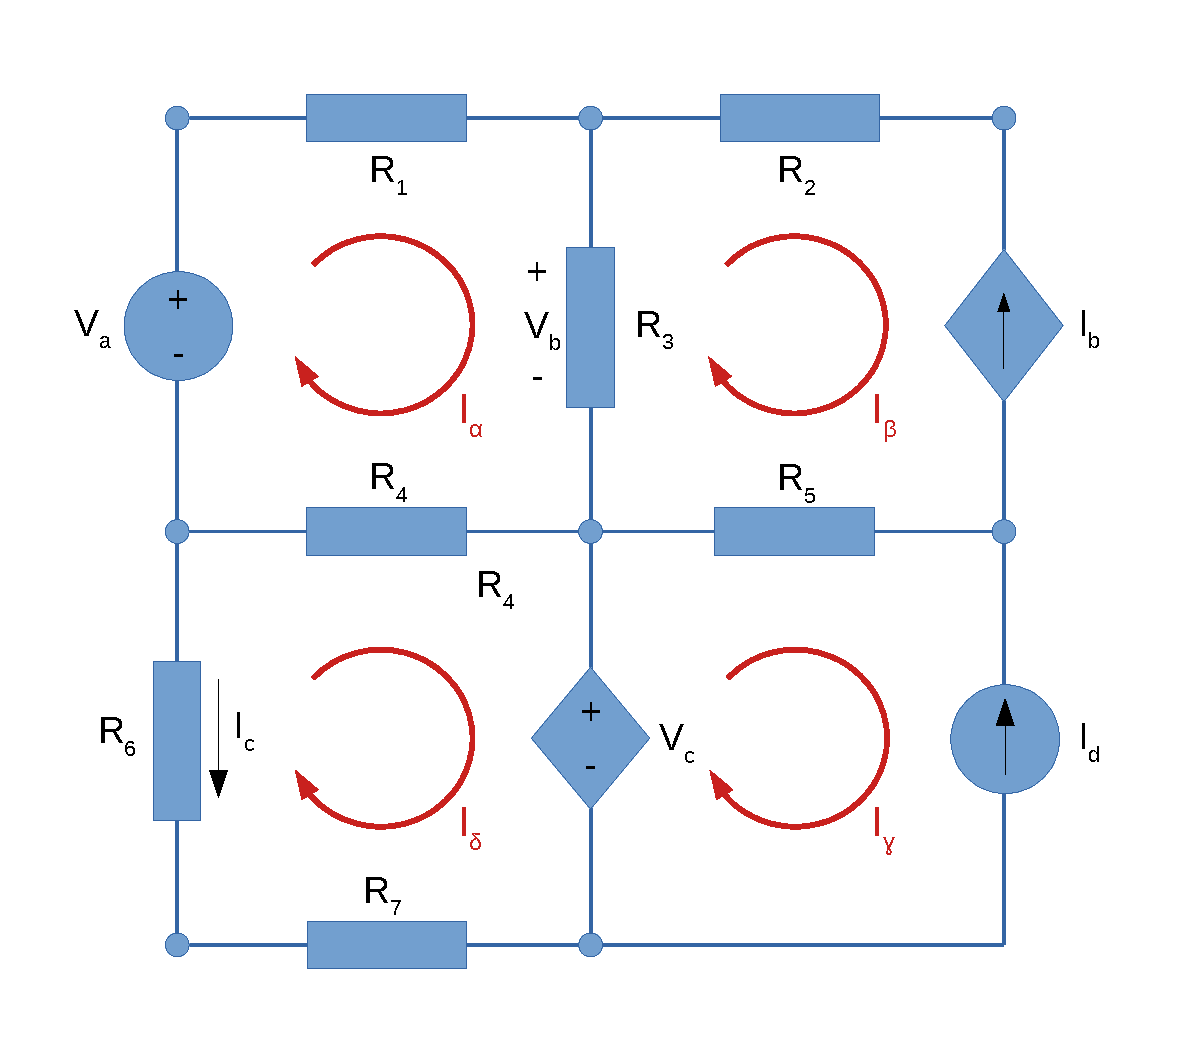
\includegraphics[width=0.45\linewidth]{CircuitMesh.pdf}
\caption{Circuit analysed with mesh currents.}
\label{fig:Circuit_Passo1}
\end{figure}

Applying the Nodal Method to this circuit leads to the following equations:

\begin{equation}
\begin{cases}
	v_1 - v_4 &= V_s;																				  \\
	\frac{1}{R_1}v_1 - (\frac{1}{R_2}+\frac{1}{R_1}+\frac{1}{R_3})v_2 + (\frac{1}{R_2})v_3 + \frac{1}{R_3}v_5 &= 0; 																						  \\
  	\frac{1}{R_2}v_2 - \frac{1}{R_2}v_3+ I_b &= 0;													  \\
  	-\frac{1}{R_1}v_1 + \frac{1}{R_1}v_2 - (\frac{1}{R_4}+\frac{1}{R_6})v_4 + \frac{1}{R_4}v_5 + \frac{1}{R_6}v_7 &= 0;			  																	  \\
	v_5 - v_8 - V_d &= 0;																			  \\
  	\frac{1}{R_5}v_5 - \frac{1}{R_5}v_6 - I_b &= 0;												  	  \\
  	-(\frac{1}{R_7}+\frac{1}{R_6})v_7 + \frac{1}{R_7}v_8 + \frac{1}{R_6}v_4 &= 0;					  \\
	v_2 - v_3 - V_b &= 0;																			  \\
  	\frac{1}{R_6}v_4 - \frac{1}{R_6}v_7 - I_d &= 0;													  \\
  	v_4 &= 0;																						  \\
  	-K_bV_b + I_b &= 0;																				  \\
  	V_d - K_cI_c &= 0.
\end{cases}
\end{equation}

Where the $2^{nd}$, $3^{rd}$, $6^{th}$ and $7^{th}$ are the equations in the respective nodes; the $1^{st}$ and $5^{th}$ are the relations imposed by the voltages soureces in those nodes; the $4^{th}$ is the supernode that bypasses $V_s$; the $8^{th}$ to $10^{th}$ are the relations between the circuit and, in order, $V_b$, $I_d$ and $v_4$; the final two equations are the ones that describe $I_b$ and $V_d$, respectivly. 
The solution to this linear system of equations is determined by Octave, plus the currents flowing in the circuit using Ohm's Law to the resistor's branches and Kirchhoff Current Law~(KCL) to the branches with voltage sources:

\begin{table}[h]
  \centering
  \begin{tabular}{|l|r|}
    \hline    
    {\bf Name} & {\bf Value [A or V]} \\ \hline
    \input{../mat/PASSO1_tab}
  \end{tabular}
  \caption{Variables in the Mesh Method. A variable preceded by @ is of type {\em current} and expressed in Ampere; other variables are of type {\em voltage} and expressed in Volt.}
  \label{tab:PASSO1}
\end{table}

All the currents were measured from the lower numbered node to the higher one; so, the direction of the current that passes through $R_6$ is, if the result is positive, from $v_4$ to $v_7$.

\subsection{Step 2: Solution for $t=0$ and $R_{eq}$}

Once found the solution for the nodes in $t<0$, the next step is to calculate the boundary conditions for the knots in the circuit, because the voltage in the nodes doesn't necessarily need to be continuos, only the difference of potencial in the capacitor, $V_c$. Therefor, a non continuos change in a power source, in this case in the voltage source $V_s$, might lead to a diferent voltage in the nodes.
Since the solution to this circuit will also be divided in natural and forced, we can use this step to evaluate the equivelent resistance of the circuit, $R_{eq}$.

To evaluate the circuit at $t=0$, we must have in mind that $V_c$ is continuos, so $V_c(0)=V_c(0^-)$. Another point to take into account is that, for the natural solution, we can ignore the sinusoidal part of $V_s$, which leaves us with $V_s=0$. In this conditions, we can say that the circuit~\ref{fig:Circuit_Base} is identical to this one:

\begin{figure}[h] \centering
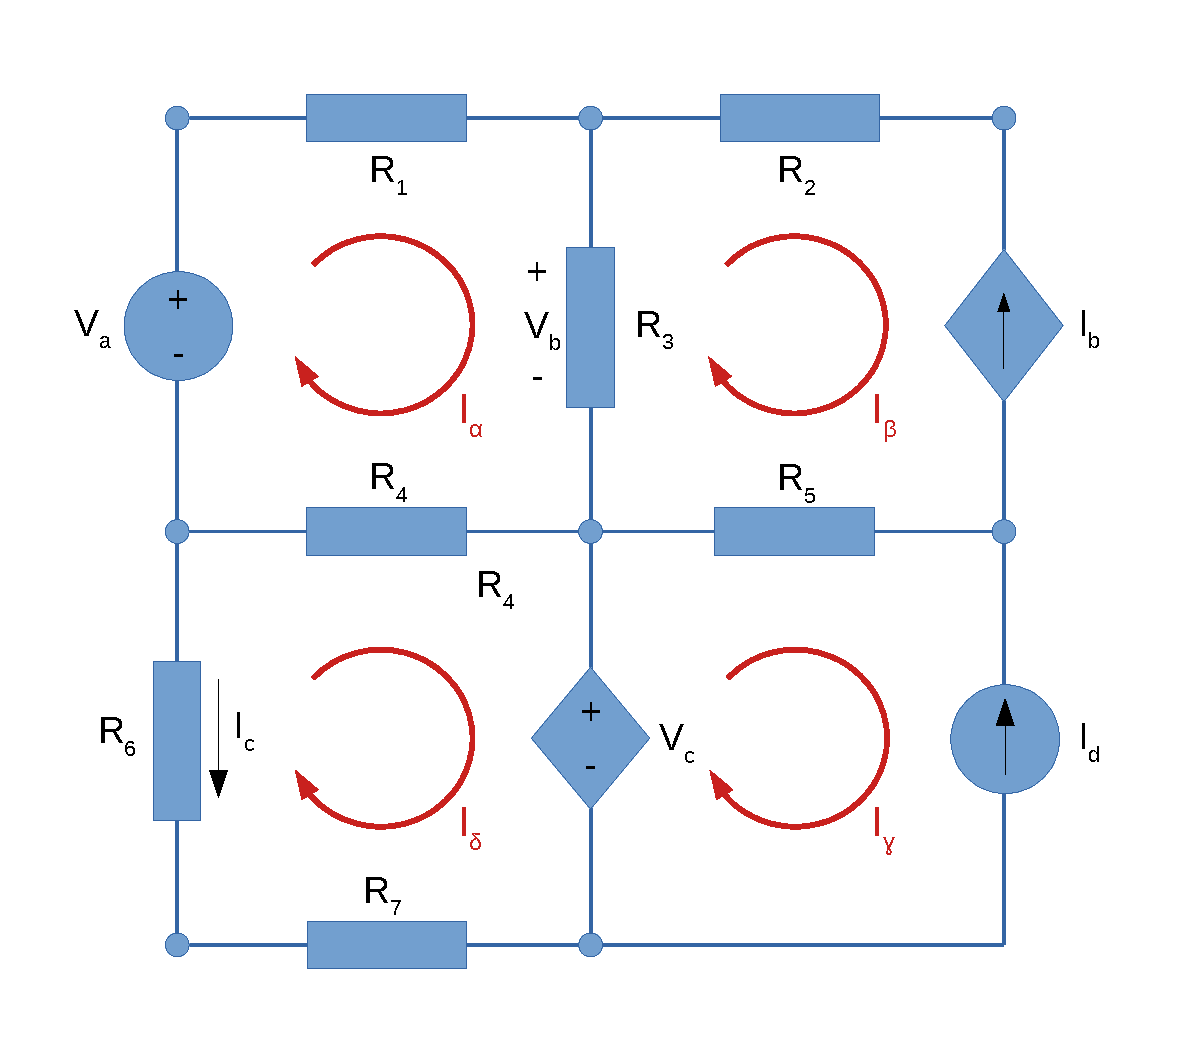
\includegraphics[width=0.45\linewidth]{CircuitMesh.pdf}
\caption{Circuit analysed with mesh currents.}
\label{fig:Circuit_Passo2}
\end{figure}

The set of equations that describe it are, using the Nodal Method:

\begin{equation}
\begin{cases}
	v_1 - v_4 &= 0;																				  	  \\
	\frac{1}{R_1}v_1 - (\frac{1}{R_2}+\frac{1}{R_1}+\frac{1}{R_3})v_2 + (\frac{1}{R_2})v_3 + \frac{1}{R_3}v_5 &= 0; \\
  	\frac{1}{R_2}v_2 - \frac{1}{R_2}v_3+ I_b &= 0;													  \\
  	-\frac{1}{R_1}v_1 + \frac{1}{R_1}v_2 - (\frac{1}{R_4}+\frac{1}{R_6})v_4 + \frac{1}{R_4}v_5 + \frac{1}{R_6}v_7 &= 0;			  																	  \\
	v_5 - v_8 - V_d &= 0;																			  \\
  	v_6 - v_8 - V_c &= 0;											  	  							  \\
  	-(\frac{1}{R_7}+\frac{1}{R_6})v_7 + \frac{1}{R_7}v_8 + \frac{1}{R_6}v_4 &= 0;					  \\
	v_2 - v_3 - V_b &= 0;																			  \\
  	\frac{1}{R_6}v_4 - \frac{1}{R_6}v_7 - I_d &= 0;													  \\
  	v_4 &= 0;																						  \\
  	-K_bV_b + I_b &= 0;																				  \\
  	V_d - K_cI_c &= 0.
\end{cases}
\end{equation}

Where the $2^{nd}$, $3^{rd}$ and $7^{th}$ are the equations in the respective nodes; the $1^{st}$, $5^{th}$ and $6^{th}$ are the relations imposed by the voltages soureces in those nodes; the $4^{th}$ is the supernode that bypasses $V_s$; the $8^{th}$ to $10^{th}$ are the relations between the circuit and, in order, $V_b$, $I_d$ and $v_4$; the final two equations are the ones that describe $I_b$ and $V_d$, respectivly. 
We note that 
\begin{equation}
	I_c = I_b + \frac{v_6-v_5}{R_5},
\end{equation}
\begin{equation}
	R_{eq} = \frac{V_c}{I_c}, \text{ and}
\end{equation}
\begin{equation}
	\tau = R_{eq}C.
\end{equation}


The solution to this linear system of equations is determined by Octave, plus the currents flowing in the circuit using Ohm's Law to the resistor's branches and Kirchhoff Current Law~(KCL) to the branches with voltage sources:

\begin{table}[h]
  \centering
  \begin{tabular}{|l|r|}
    \hline    
    {\bf Name} & {\bf Value [A or V]} \\ \hline
    \input{../mat/PASSO2_tab}
  \end{tabular}
  \caption{Variables in the Mesh Method. A variable preceded by @ is of type {\em current} and expressed in Ampere; other variables are of type {\em voltage} and expressed in Volt.}
  \label{tab:PASSO2}
\end{table}


\subsection{Step 3: Natural Solution for $t>0$}

Using $R_{eq}$ and $v_6$ from the previous step we can compute the natural solution of $v_6(t)$:

\begin{equation}
	
	v_6(t) =& v_6(+\infty) - (v_6(+\infty) - v_6(0))e^{-\frac[1}[\tau}t}		\\
	v_6(t) =& v_6(0))e^{-\frac[1}[\tau}t}, \text{ dado que } (v_6(+\infty) = 0.
	
\end{equation}

Using Octave to plot this equation gives us:

\begin{figure}[h] \centering
\includegraphics[width=0.45\linewidth]{../mat/PASSO3.eps}
\caption{Natural solution of $v_6(t)$.}
\label{fig:TEO_NAT_SOL}
\end{figure}

\subsection{Step 4: Forced Solution for $t>0$}

Since $V_s$ is a sinusoidal source in $t>0$, we can perform a complex analysis, replacing all the componets for their impedances. In this case, only the capacitor changes (since all resistors have the same impedance):

\begin{equation}
	
	Z_c = \frac{j\omegaC}
	
\end{equation}

Where $\omega$ is the frequency ($1k rads^{-1}$).
Saying that $V_s = 1$ to calculate the phasors relative to $V_s$ and using the Nodal Method we arive to a set of equations:

\begin{equation}
\begin{cases}
	v_1 - v_4 &= 1;																				  	  \\
	\frac{1}{R_1}v_1 - (\frac{1}{R_2}+\frac{1}{R_1}+\frac{1}{R_3})v_2 + (\frac{1}{R_2})v_3 + \frac{1}{R_3}v_5 &= 0; \\
  	\frac{1}{R_2}v_2 - \frac{1}{R_2}v_3+ I_b &= 0;													  \\
  	-\frac{1}{R_1}v_1 + \frac{1}{R_1}v_2 - (\frac{1}{R_4}+\frac{1}{R_6})v_4 + \frac{1}{R_4}v_5 + \frac{1}{R_6}v_7 &= 0;			  																	  \\
	v_5 - v_8 - V_d &= 0;																			  \\
  	\frac{1}{R_5}v_5 - (\frac{1}{R_5} + j\omegaC)v_6 + (j\omegaC)v_8- I_b &= 0;						  \\
  	-(\frac{1}{R_7}+\frac{1}{R_6})v_7 + \frac{1}{R_7}v_8 + \frac{1}{R_6}v_4 &= 0;					  \\
	v_2 - v_3 - V_b &= 0;																			  \\
  	\frac{1}{R_6}v_4 - \frac{1}{R_6}v_7 - I_d &= 0;													  \\
  	v_4 &= 0;																						  \\
  	-K_bV_b + I_b &= 0;																				  \\
  	V_d - K_cI_c &= 0.
\end{cases}
\label{eq:PASSO4}
\end{equation}

Where the $2^{nd}$, $3^{rd}$, $6^{th}$ and $7^{th}$ are the equations in the respective nodes; the $1^{st}$ and $5^{th}$ are the relations imposed by the voltages soureces in those nodes; the $4^{th}$ is the supernode that bypasses $V_s$; the $8^{th}$ to $10^{th}$ are the relations between the circuit and, in order, $V_b$, $I_d$ and $v_4$; the final two equations are the ones that describe $I_b$ and $V_d$, respectivly. 

The solution to this linear system of equations is determined by Octave:

\begin{table}[h]
  \centering
  \begin{tabular}{|l|r|}
    \hline    
    {\bf Name} & {\bf Value} \\ \hline
    \input{../mat/PASSO4_tab}
  \end{tabular}
  \caption{Variables in the Nodal Method. Variables are adimentional.}
  \label{tab:PASSO4}
\end{table}

The forced solution of $v_6(t)$ is given by $v_6(t) = V_s(t)*Pv_6$.

\subsection{Step 5: Total Solution for $t\in [-5,20]ms$}

The total solution of $v_6$ will be the solution from step 1 for $t\in [-5,0[ms$ and the sum of the natural solution and forced solution for $t\in [0,20]ms$
The plot given by Octave is:

\begin{figure}[h] \centering
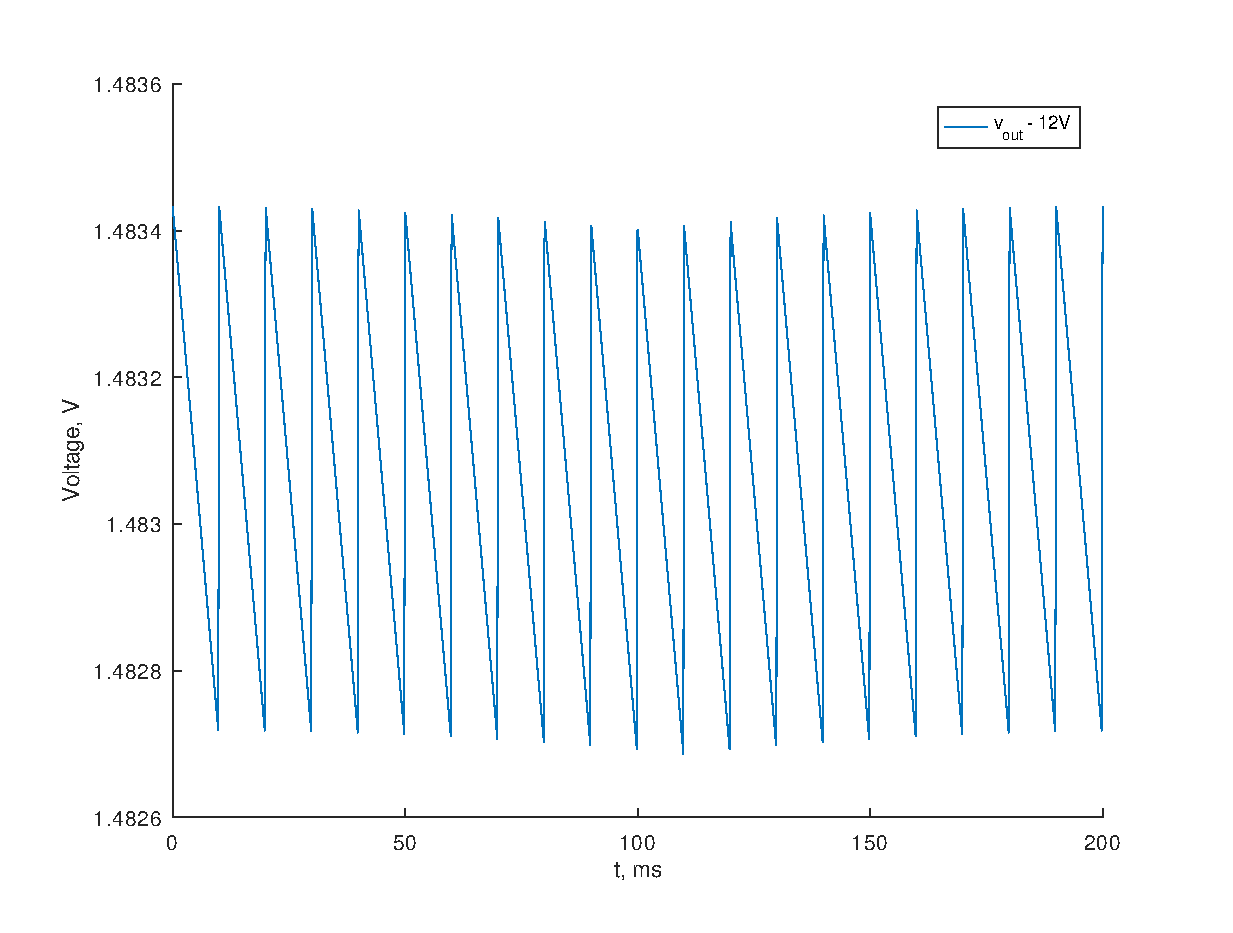
\includegraphics[width=0.45\linewidth]{../mat/PASSO5.eps}
\caption{Total solution of $v_6(t)$ and $V_s(t)$.}
\label{fig:TEO_TOT_SOL}
\end{figure}

\subsection{Step 6: Frequency Response of $v_6$ and $V_c$}

In this subsection is made an analysis of the frequency response of $v_6$ and $V_c$ in order to $V_s$. for that we need to solve the same system as in step 4 (equation \ref{eq:PASSO4}), with $\omega$ as a parameter. The magnitude (absolute value of the complex vectors) and phase (angle of the complex vectors is ploted using Octave:

\begin{figure}[h] \centering
\includegraphics[width=0.45\linewidth]{../mat/PASSO6-AMPLITUDE.eps}
\caption{Magnitude responce of $V_s$, $v_6(t)$, $V_c(t)$ and $v_8$.}
\label{fig:TEO_MAG}
\end{figure}

\begin{figure}[h] \centering
\includegraphics[width=0.45\linewidth]{../mat/PASSO6-ANGULO.eps}
\caption{Angle responce of $V_s$, $v_6(t)$, $V_c(t)$ and $v_8$.}
\label{fig:TEO_ANG}
\end{figure}

The results of $V_s$ are to be expected, since $\frac{V_s}{V_s}=1$.
The results of $V_c$ are also expected, since a capacitor is a low pass filter and this plots match to the ones of the classes.
The results of $v_6$ are, at first glance, unnexpected, since we are used to suppose that $v_6 \to 0$; but in fact what happens is that $V_c \to 0 \Rightarrow v_6 - v_8 \to 0$. Because the phase response of $v_8$ is constant, $v_6 - v_8 \to 0 \Rightarrow v_6 \to v_8$.





\newpage
\section{Simulation Analysis }
\label{sec:simulation}

\subsection{Operating Point Analysis for $t<0$}

Table~\ref{tab:SIM_PASSO1} shows the simulated operating point results for the circuit under analysis for $t<0$.
%Colocar a tabela 
\begin{table}[h]
  \centering
  \begin{tabular}{|l|r|}
    \hline    
    {\bf Name} & {\bf Value [A or V]} \\ \hline
    \input{../sim/PASSO1_tab}
  \end{tabular}
  \caption{Operating point for $t<0$. A variable preceded by @ is of type {\em current}
    and expressed in Ampere; other variables are of type {\it voltage} and expressed in
    Volt.}
  \label{tab:SIM_PASSO1}
\end{table}

It is important to notice that it has been necessary to implement an extra test voltage sorce  between the node 7 and $R_6$ providing 0V so that is does not interfere with the rest of the circuit and enable us to measure the voltage $V_d$ flowing in the dependent source. Therefore, this creation does not change any results and it is only based on the Ngspice requirements to define a current controlled voltage source.

Compared to the theoretical analysis the simulation showed practically identical results, except for a small divergence in the last decimal place that probably occurs when Ngspice rounds the numbers. Thus, the maximum relative error is $10^{-5}$. It is worth mentioning that Ngspice software also uses the same mathematical methods as octave to find results, hence, this result was already expected.


\subsection{Operating Point Analysis for $t=0$}

The circuit was simulated using an operating point analysis with $V_s(0)=0$ and replacing que capacitor with a voltage source $V_c=V(6)-V(8)$ as these were obtained in the previous step. This step in required to compute the boundary conditions that ensure the continuity in the capacitor. Table~\ref{tab:SIM_PASSO2} shows the results of the simulation. Notice that:  \begin{equation}
R_{eq}=\frac{V_{c}}{I_{c}}
\end{equation}

\begin{table}[h]
  \centering
  \begin{tabular}{|l|r|}
    \hline    
    {\bf Name} & {\bf Value [A or V]} \\ \hline
    \input{../sim/PASSO2_tab}
  \end{tabular}
  \caption{Operating point for $t=0$. A variable preceded by @ is of type {\em current}
    and expressed in Ampere; other variables are of type {\it voltage} and expressed in
    Volt.}
  \label{tab:SIM_PASSO2}
\end{table}

\subsection{Natural Solution for $V_6$}

In order to study the natural response of the circuit in the interval [0,20]ms, a transient analysis was made, using the results for $V_6$ and $V_8$ computed in the previous step. Figure \ref{fig:SIM_NAT_SOL} shows the results for the natural solution for $V_6$.

\begin{figure}[h] \centering
\vspace{-3cm}
\includegraphics[height=10cm]{../sim/trans.pdf}
\caption{Natural solution of $v_6(t)$.}
\label{fig:SIM_NAT_SOL}
\end{figure}

\newpage
\subsection{Total Solution for $V_6$}

The results obtained in the last section were used to make this analysis,but considering $V_s$ a sinusoidal voltage source with f=1kHz. The total response of the circuit is the result of summing the natural analysis with the forced one (natural + forced). 
Figure \ref{fig:SIM_TOT_SOL} shows the total transient analysis results for $v_6(t)$.

\begin{figure}[h] \centering
\includegraphics[height=12cm]{../sim/trans2.pdf}
\caption{$V_s$ and total solution of $v_6(t)$.}
\label{fig:SIM_TOT_SOL}
\end{figure}

\newpage
\subsection{Frequency Response}


In this section, the frequency range considered to analyze the frequency response in node 6 is from 0.1 Hz to 1 MHz. The figures show the magnitude and phase of the frequency response for $V_s$, $V_c$ and $V_6$.

\begin{figure}[h] \centering
\vspace{-3cm}
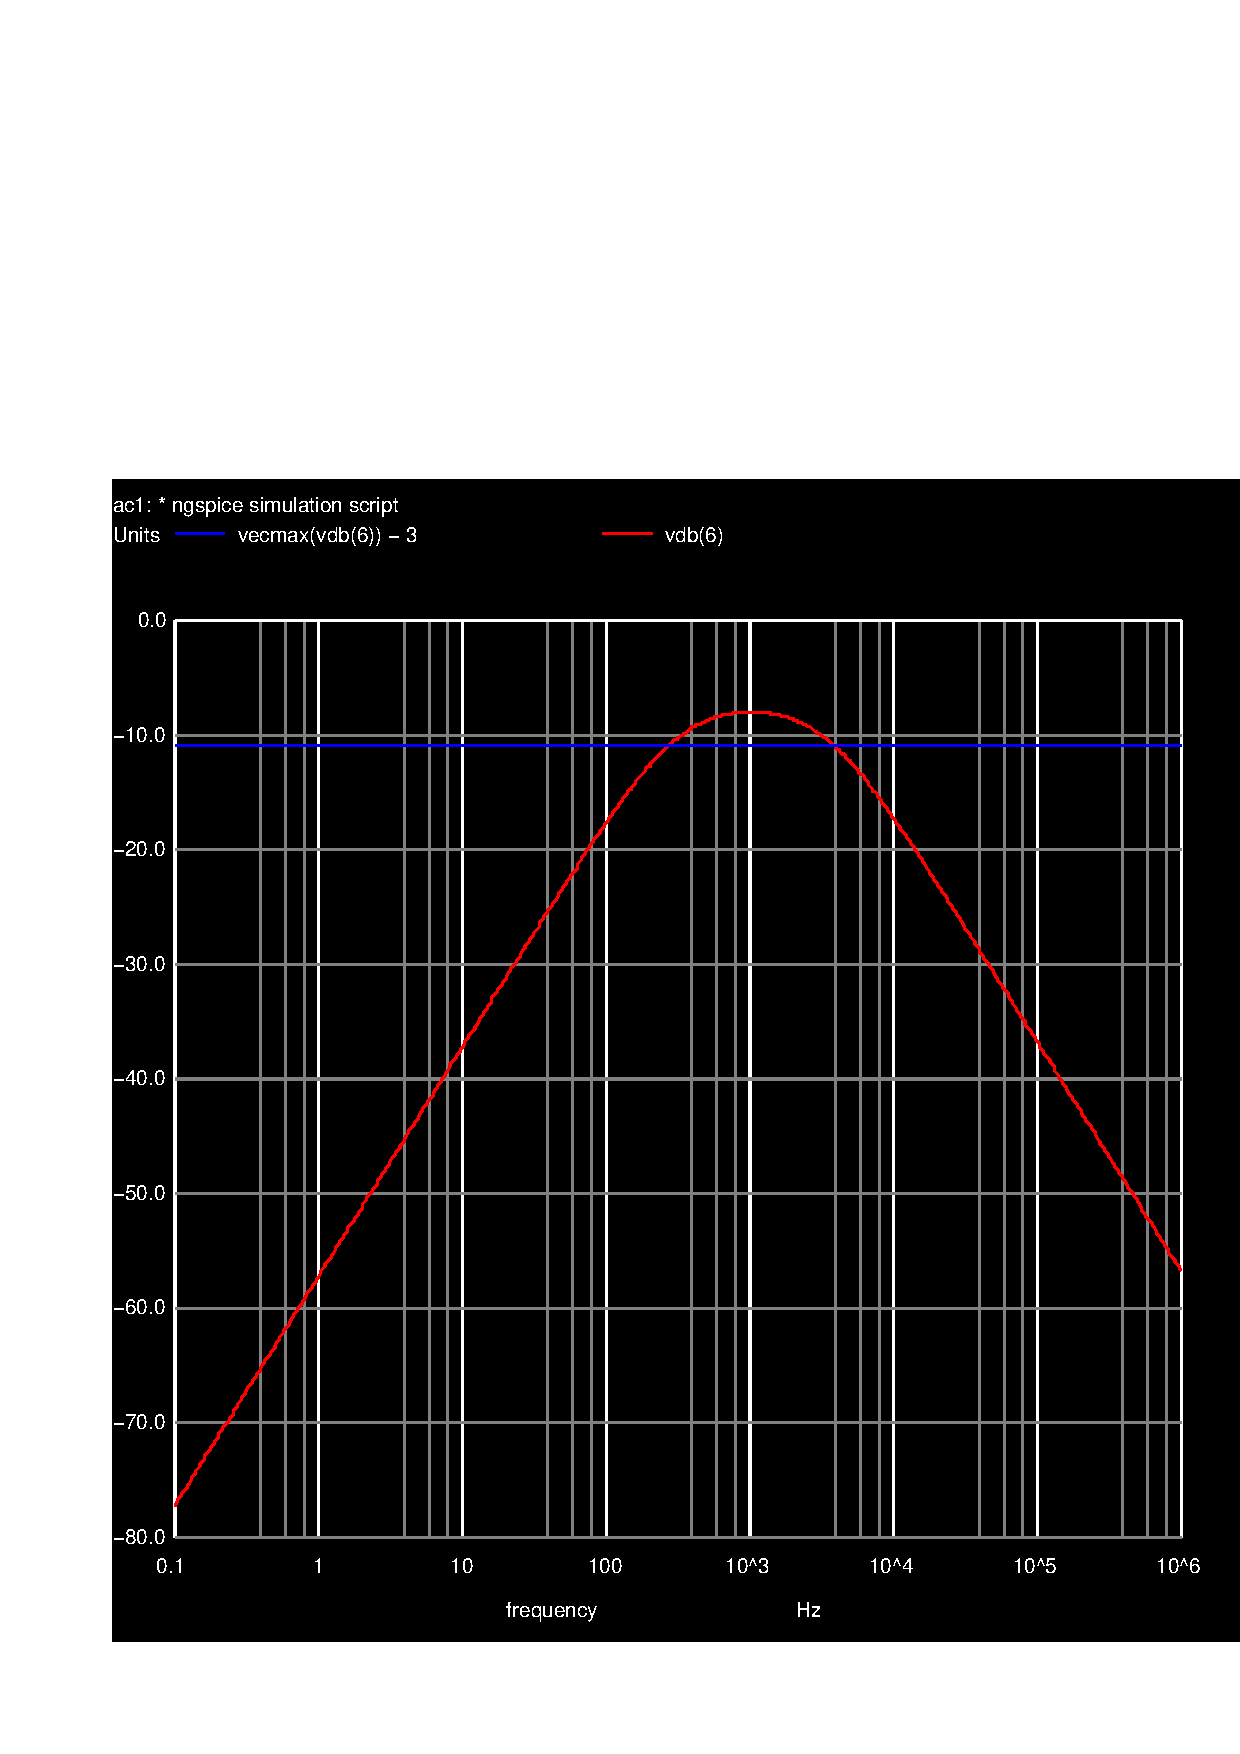
\includegraphics[height=10cm]{../sim/db.pdf}
\caption{Magnitude response of $v_6(t)$, $V_s$ and $V_c(t)$.}
\label{fig:SIM_MAG}
\end{figure}

\begin{figure}[h] \centering
\vspace{-3cm}
\includegraphics[height=10cm]{../sim/ph.pdf}
\caption{Angle response of $v_6(t)$, $V_s$ and $V_c(t)$.}
\label{fig:SIM_ANG}
\end{figure}

When comparing the graphics obtained in Ngspice and Octave, the similarity between the results is noticeable and small differences can be explained by approximation errors.




\newpage
\section{Conclusion}
\label{sec:conclusion}

All things considered, an audio amplifier with the smallest number of components that allows a greater gain in voltage was the main objective of this laboratory. A theoretically and simulated model was created to analyze this amplifier and see how it works. \par
Using Octave as the theoretical analysis and Ngspice for the simulation, a very discrepant results were observed between the two. The main cause of this problem is due of the transistor models used in Ngspice that is more complex than Octave models. Transistors in Ngspice makes it impossible to get the same results because of non-linearity components.\par
It is possible to say that the theoretical model had a good result even with its low complexity, but only for low frequencies, as shown in figures~\ref{fig:SIM_OUT}, \ref{fig:SIM_PH}, \ref{fig:MAT_OUT}, \ref{fig:MAT_PH}. This is possibly due to the rise of second and higher order derivatives of the function that describe the circuit and in the theoretical analysis are not considered. But it shows that Ngspice has results more like reality due to more accurate models and components.

The tables with the results are the following:

%%	DC

\begin{table}[h]
\centering
\begin{minipage}[t]{0.35\linewidth}
 	 \begin{tabular}[t]{|l|r|}
 	   \hline    
 	   {\bf Name} & {\bf Value} \\ \hline
 	   \input{../mat/MAT_DC_tab}
 	 \end{tabular}
\end{minipage}
\begin{minipage}[t]{0.40\linewidth}
  	\begin{tabular}[t]{|l|r|}
    	\hline    
   		{\bf Name} & {\bf Value} \\ \hline
    	\input{../sim/SIM_DC_tab}
  	\end{tabular}
\end{minipage}

  	\caption{Results in Octave and NGSpice, respectivily. The variables are of type {\it voltage} and expressed in Volt (As shown in Tables \ref{tab:TEO_DC} and \ref{tab:SIM_DC}).}
\end{table}

%%	Impedance

\begin{table}[h]
\centering
\begin{minipage}[t]{0.47\linewidth}
 	 \begin{tabular}[t]{|l|r|}
 	   \hline    
 	   {\bf Name} & {\bf Value} \\ \hline
 	   \input{../mat/MAT_IMP_tab}
 	 \end{tabular}
\end{minipage}
\begin{minipage}[t]{0.47\linewidth}
  	\begin{tabular}[t]{|l|r|}
    	\hline    
   		{\bf Name} & {\bf Value} \\ \hline
    	\input{../sim/SIM_ZIN_tab}
  	\end{tabular}
	\begin{tabular}[t]{|l|r|}
    	\hline    
   		{\bf Name} & {\bf Value [A or V]} \\ \hline
    	\input{../sim/SIM_ZOUT_tab}
  	\end{tabular}
\end{minipage}

\caption{Results in Octave and NGSpice, respectivily. NGSpice values are of of type {\it impedance} and expressed in Ohm; variables preceded by \# are of type {\it impedance} and expressed in Ohm; other variables are adimentional. (As shown in Tables \ref{tab:TEO_IMP}, \ref{tab:SIM_ZIN} and \ref{tab:SIM_ZOUT})}
\end{table}

%%	AC

\begin{table}[h]
\centering
\begin{minipage}[t]{0.40\linewidth}
 	 \begin{tabular}[t]{|l|r|}
 	   \hline    
 	   {\bf Name} & {\bf Value} \\ \hline
 	   \input{../mat/MAT_GAIN_tab}
 	 \end{tabular}
\end{minipage}
\begin{minipage}[t]{0.45\linewidth}
  	\begin{tabular}[t]{|l|r|}
    	\hline    
   		{\bf Name} & {\bf Value} \\ \hline
    	\input{../sim/SIM_RESULTS_tab}
  	\end{tabular}
\end{minipage}

  	\caption{Results in Octave and NGSpice, respectivily. Merit is in {\it per voltage per cost} and expressed in Volt$^{-1}$UC$^{-1}$; $f1 - f2$ is of the type {\it frequency} and expressed in Hz; other variables are adimentional. (As shown in Tables \ref{tab:TEO_RES} and \ref{tab:SIM_RES})}
\end{table}


The Merit result was 260.6748 $V^{-1}uc^{-1}$ by Ngspice. It was agreed by the members of the group that the main goal of task was completed.

\newpage
The obtained plot with NGSpice and Octave are the following:

\begin{figure}[h] \centering
	\vspace{-3cm}
	\includegraphics[height=12cm]{../sim/ampdb.pdf}
	\caption{NGSpice plot:$db(v_{out})$ and $max(db(v_{out}))-3$.}
	\label{fig:MAT_OUT}
\end{figure}

\begin{figure}[h] \centering
	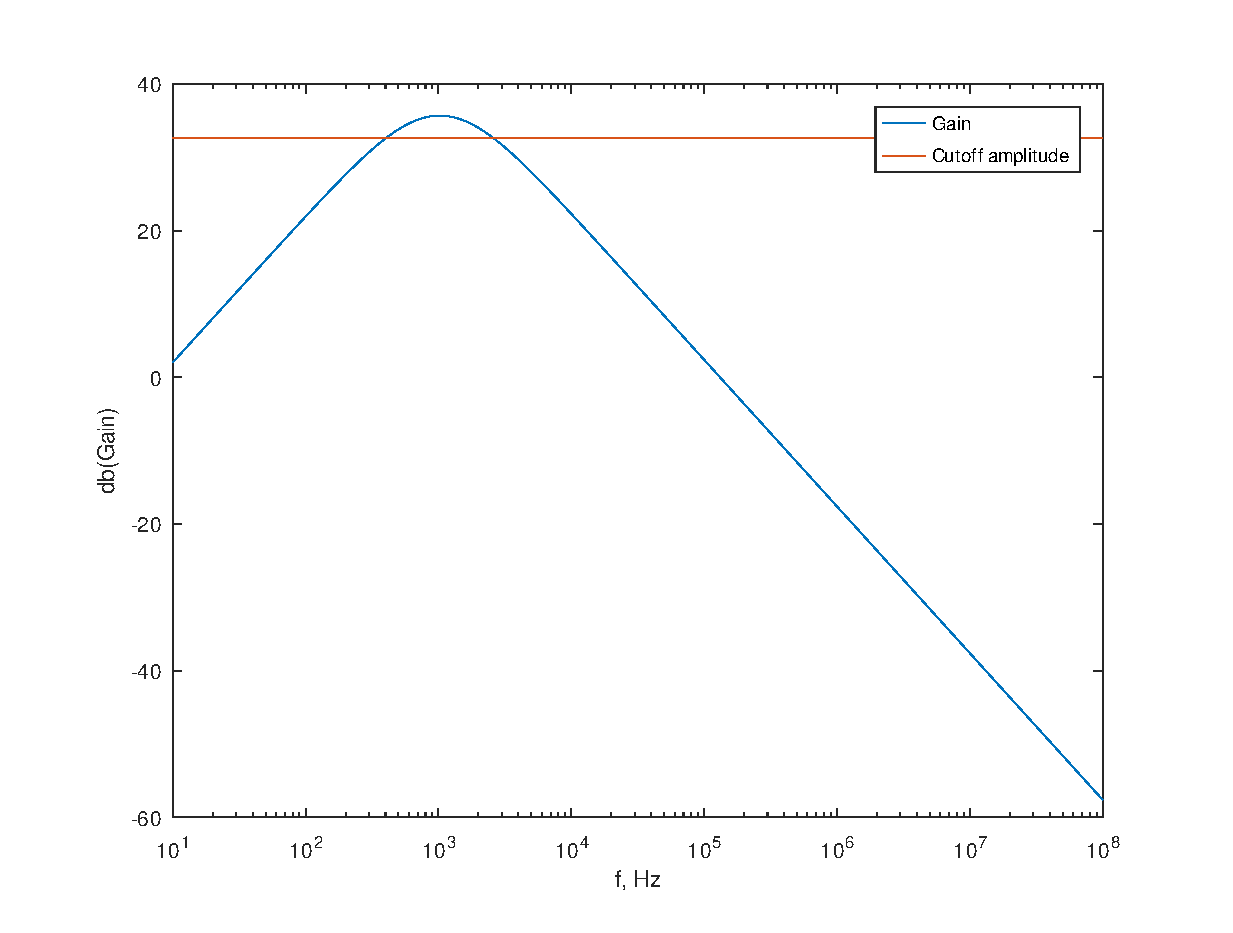
\includegraphics[height=8cm]{MAT_AB_AMP.eps}
	\caption{Octave plot:$db(v_{out})$ and $max(db(v_{out}))-3$.}
	\label{fig:SIM_OUT}
\end{figure}

\newpage

\begin{figure}[h] \centering
	\vspace{-3cm}
	\includegraphics[height=12cm]{../sim/phdb.pdf}
	\caption{NGSpice plot: Phasor of $v_{out}$, rad}
	\label{fig:MAT_PH}
\end{figure}

\begin{figure}[h] \centering
	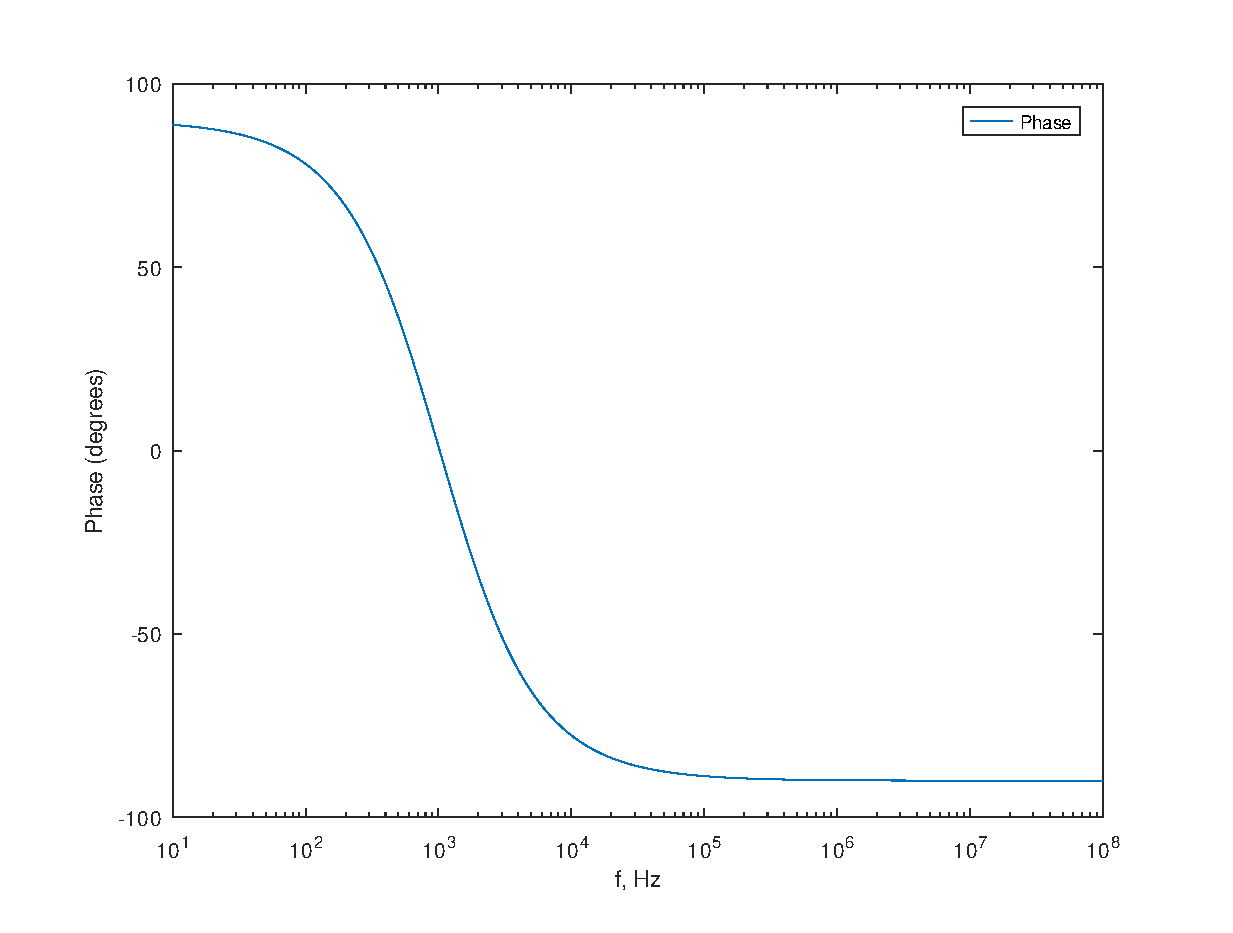
\includegraphics[height=8cm]{MAT_AB_PH.eps}
	\caption{Octave plot: Phasor of $v_{out}$, rad}
	\label{fig:SIM_PH}
\end{figure}

\newpage

\begin{figure}[h] \centering
	\vspace{-3cm}
	\includegraphics[height=12cm]{../sim/trans.pdf}
	\caption{NGSpice plot: $v_{in}$ and $v_{out}$.}
\end{figure}

\begin{figure}[h] \centering
	\vspace{-3cm}
	\includegraphics[height=12cm]{../sim/amp.pdf}
	\caption{$ \left | v_{out}/v_{in} \right |$.}
	\vspace{-2cm}
\end{figure}

%\cleardoublepage

% ----------------------------------------------------------------------
%  Bibliography
% ----------------------------------------------------------------------
%\addcontentsline{toc}{section}{\bibname}
%\bibliographystyle{abbrvunsrtnat} % <<<<< SELECT IF USING REFERENCES BY NUMBER (CITATION ORDER)
%\bibliography{../../../BIBfile.bib}

% ----------------------------------------------------------------------
\end{document}
% ----------------------------------------------------------------------

